\chapter[\itshape Descriptive Notes]{
    
\includegraphics[width=9.3cm]{viking-tales/046}}

\phantomsection\label{house}
\emph{House.} In a rich Norseman's home were many buildings. The finest
and largest was the great feast hall. Next were the bower, where the
women worked, and the guest house, where visitors slept. Besides these
were storehouses, stables, work-shops, a kitchen, a sleeping-house for
thralls. All these buildings were made of heavy, hewn logs, covered with
tar to fill the cracks and to keep the wood from rotting. The ends of
the logs, the door-posts, the peaks of gables, were carved into shapes
of men and animals and were painted with bright colors. These gay
buildings were close together, often set around the four sides of a
square yard. That yard was a busy and pleasant place, with men and women
running across from one bright building to another. Sometimes a high
fence with one gate went around all this, and only the tall, carved
peaks of roofs showed from the outside.

\phantomsection\label{names}
\noindent\emph{Names.} An old Norse story says: ``Most men had two names
in one, and thought it likeliest to lead to long life and good luck to
have double names.'' To be called after a god was very lucky. Here are
some of those double names with their meanings: ``Thorstein'' means
Thor's stone; ``Thorkel'' means Thor's fire; ``Thorbiorn'' means Thor's
bear; ``Gudbrand'' means Gunnr's sword (Gunnr was one of the
Valkyrias\footnote{See note about Valkyrias on
page~\pageref{valkyrias}.}); ``Gunnbiorn'' means Gunnr's bear; ``Gudrid''
means Gunnr's rider; ``Gudrod'' means Gunnr's land-clearer. (Most of the
land in old Norway was covered with forests. When a man got new land he
had to clear off the trees.) In those olden days a man did not have a
surname that belonged to everyone in his family. Sometimes there were
two or three men of the same name in a neighborhood. That caused
trouble. People thought of two ways of making it easy to tell which man
was being spoken of. Each was given a nickname. Suppose the name of each
was Haki. One would be called Haki the Black because he had black hair.
The other would be called Haki the Ship-chested because his chest was
broad and strong. These nicknames were often given only for the fun of
it. Most men had them,--Eric the Red, Leif the Lucky, Harald Hairfair,
Rolf Go-afoot. The other way of knowing one Haki from the other was to
tell his father's name. One was Haki, Eric's son. The other was Haki,
Halfdan's son. If you speak these names quickly, they sound like Haki
Ericsson and Haki Halfdansson. After a while they were written like
that, and men handed them on to their sons and daughters. Some names
that we have nowadays have come down to us in just that way--Swanson,
Anderson, Peterson, Jansen. There was another reason for these last
names: a man was proud to have people know who his father was.

\phantomsection\label{drinking-horns}
\noindent\emph{Drinking-horns.} The Norsemen had few cups or goblets.
They used instead the horns of cattle, polished and trimmed with gold or
silver or bronze. They were often very beautiful, and a man was almost as
proud of his drinking-horn as of his sword.

\phantomsection\label{tables}
\noindent\emph{Tables.} Before a meal thralls brought trestles into the
feast hall and set them before the benches. Then they laid long boards
across from trestle to trestle. These narrow tables stretched all along
both sides of the hall. People sat at the outside edge only. So the
thralls served from the middle of the room. They put baskets of bread and
wooden platters of meat upon these bare boards. At the end of the meal
they carried out tables and all, and the drinking-horns went round in a
clean room.

\phantomsection\label{beds}
\noindent\emph{Beds.} Around the sides of the feast hall were shut-beds.
They were like big boxes with doors opening into the hall. On the floor
of this box was straw with blankets thrown over it. The people got into
these beds and closed the doors and so shut themselves in. Olaf's men
could have set heavy things against these doors or have put props
against them. Then the people could not have got out; for on the other
side of the bed was the thick outside wall of the feast hall, and there
were no windows in it.

\phantomsection\label{feast-hall}
\noindent\emph{Feast Hall.} The feast hall was long and narrow, with a
door at each end. Down the middle of the room were flat stones in the
dirt floor. Here the fires burned. In the roof above these fires were
holes for the smoke to go out, but some of it blew about the hall, and
the walls and rafters were stained with it. But it was pleasant wood
smoke, and the Norsemen did not dislike it. There were no large windows
in a feast hall or in any other Norse building. High up under the eaves
or in the roof itself were narrow slits that were called wind's-eyes.
There was no glass in them, for the Norsemen did not know how to make it;
but there were, instead, covers made of thin, oiled skin. These were put
into the wind's-eyes in stormy weather. There were covers, too, for the
smoke-holes. The only light came through these narrow holes, so on dark
days the people needed the fire as much for light as for warmth.

\phantomsection\label{foster-father}
\noindent\emph{Foster-father.} A Norse father sent his children away from
home to grow up. They went when they were three or four years old and
stayed until they were grown. The father thought: ``They will be better
so. If they stayed at home, their mother would spoil them with much
petting.''

\phantomsection\label{foster-brothers}
\noindent\emph{Foster-brothers.} When two men loved each other very much
they said, ``Let us become foster-brothers.''

Then they went and cut three long pieces of turf and put a spear into
the ground so that it held up the strips of turf like an arch. Runes
were cut on the handle of the spear, telling the duties of
foster-brothers. The two men walked under this arch, and each made a
little cut in his palm. They knelt and clasped hands, so that the blood
of the two flowed together, and they said, ``Now we are of one blood.''

Then each made this vow: ``I will fight for my foster-brother whenever
he shall need me. If he is killed before I am, I will punish the man who
did it. Whatever things I own are as much my foster-brother's as mine. I
will love this man until I die. I call Odin and Thor and all the gods to
hear my vow. May they hate me if I break it!''

\phantomsection\label{ran}
\noindent\emph{Ran.} Ran was the wife of Aegir, who was god of the sea.
They lived in a cave at the bottom of the ocean. Ran had a great net, and
she caught in it all men who were shipwrecked and took them to her cave.
She also caught all the gold and rich treasures that went down in ships.
So her cave was filled with shining things.

\phantomsection\label{valkyrias}
\noindent\emph{Valkyrias.} These were the maidens of Odin. They waited
on the table in Valhalla. But whenever a battle was being fought they
rode through the air on their horses and watched to see what warriors
were brave enough to go to Valhalla. Sometimes during the fight a man
would think that he saw the Valkyrias. Then he was glad; for he knew that
he would go to Valhalla.

An old Norse story says this about the Valkyrias: ``With lightning
around them, with bloody shirts of mail, and with shining spears they
ride through the air and the ocean. When their horses shake their manes,
dew falls on the deep valleys and hail on the high forests.''

\phantomsection\label{odins-ravens}
\noindent\emph{Odin's Ravens.} Odin had a great throne in his palace in
Asgard. When he sat in it he could look all over the world. But it was so
far to see that he could not tell all of the things that were happening.
So he had two ravens to help him. An old Norse story tells this about
them: ``Two ravens sit on Odin's shoulders and whisper in his ears all
that they have heard and seen. He sends them out at dawn of day to see
over the whole world. They return at evening near meal time. This is why
Odin knows so many things.''

\phantomsection\label{reykjavik}
\noindent\emph{Reykjavik.} Reykjavik means ``smoky sea.'' Ingolf called
it that because of the steaming hot-springs by the sea. The place is
still called Reykjavik. A little city has grown up there, the only city
in Iceland. It is the capital of the country.

\phantomsection\label{peace-bands}
\noindent\emph{Peace-bands.} A Norseman always carried his sword, even at
a feast; for he did not know when he might need it. But when he went
somewhere on an errand of peace and had no quarrel he tied his sword
into its scabbard with white bands that he called peace-bands. If all at
once something happened to make him need his sword, he broke the
peace-bands and drew it out.

\phantomsection\label{eskimos}
\noindent\emph{Eskimos.} Now, the Eskimos live in Greenland and Alaska
and on the very northern shores of Canada. But once they lived farther
south in pleasanter lands. After a while the other Indian tribes began to
grow strong. Then they wanted the pleasant land of the Eskimos and the
seashore that the Eskimos had. So they fought again and again with those
people and won and drove them farther north and farther north. At last
the Eskimos were on the very shores of the cold sea, with the Indians
still pushing them on. So some of them got into their boats and rowed
across the narrow water and came to Greenland and lived there. Some
people think that these things happened before Eric found Greenland. In
that case he found Eskimos there; and Thorfinn saw red Indians in
Wineland. Other people think that this happened after Eric went to
Greenland. If that is true, he found an empty land, and it was Eskimos
that Thorfinn saw in Wineland.

\chapter[\itshape Suggestions to Teachers]{
    
\includegraphics[width=9.3cm]{viking-tales/047}}

\lettrine{P}{ossibly} this book seems made up of four or five
disconnected stories. They are, however, strung upon one thread,--the
westward emigration from Norway. The story of Harald is intended to serve
in two ways towards the working out of this plot. It gives the general
setting that continues throughout the book in costume, houses, ideals,
habits. It explains the cause of the emigration from the mother country.
It is really an introductory chapter. As for the other stories, they are
distinctly steps in the progress of the plot. A chain of islands loosely
connects Norway with America,--Orkneys and Shetlands, Faroes, Iceland,
Greenland. It was from link to link of this chain that the Norsemen
sailed in search of home and adventure. Discoveries were made by
accident. Ships were driven by the wind from known island to unknown.
These two points,--the island connection that made possible the long
voyage from Norway to America, and the contribution of storm to
discovery,--I have stated in the book only dramatically. I emphasize them
here, hoping that the teacher will make sure that the children see them,
and possibly that they state them abstractly.

Let me speak as to the proper imaging of the stories. I have not often
interrupted incident with special description, not because I do not
consider the getting of vivid and detailed images most necessary to full
enjoyment and to proper intellectual habits, but because I trusted to
the pictures of this book and to the teacher to do what seemed to me
inartistic to do in the story. Some of these descriptions and
explanations I have introduced into the book in the form of notes,
hoping that the children in turning to them might form a habit of
insisting upon full understanding of a point, and might possibly, with
the teacher's encouragement, begin the habit of reference reading.

The landscape of Norway, Iceland, and Greenland is wonderful and will
greatly assist in giving reality and definiteness to the stories.
Materials for this study are not difficult of access. Foreign colored
photographs of Norwegian landscape are becoming common in our art
stores. There are good illustrations in the geographical works referred
to in the book list. These could be copied upon the blackboard. There
are three books beautifully illustrated in color that it will be
possible to find only in large libraries,--``Coast of Norway,'' by
Walton; ``Travels in the Island of Iceland,'' by Mackenzie; ``Voyage en
Islande et au Gröenland,'' by J. P. Gaimard. If the landscape is studied
from the point of view of formation, the images will be more accurate
and more easily gained, and the study will have a general value that
will continue past the reading of these stories into all work in
geography.

Trustworthy pictures of Norse houses and costumes are difficult to
obtain. In ``Viking Age'' and ``Story of Norway,'' by Boyesen (G. P.
Putnam's Sons, New York), are many copies of Norse antiquities in the
fashion of weapons, shield-bosses, coins, jewelry, wood-carving. These
are, of course, accurate, but of little interest to children. Their
chief value lies in helping the teacher to piece together a picture that
she can finally give to her pupils.

Metal-working and wood-carving were the most important arts of the
Norse. If children study products of these arts and actually do some of
the work, they will gain a quickened sympathy with the people and an
appreciation of their power. They may, perhaps, make something to merely
illustrate Norse work; for instance, a carved ship's-head, or a copper
shield, or a wrought door-nail. But, better, they may apply Norse ideas
of form and decoration and Norse processes in making some modern thing
that they can actually use; for instance, a carved wood pin-tray or a
copper match holder. This work should lead out into a study of these
same industries among ourselves with visits to wood-working shops and
metal foundries.

Frequent drawn or painted illustration by the children of costumes,
landscapes, houses, feast halls, and ships will help to make these
images clear. But dramatization will do more than anything else for the
interpreting of the stories and the characters. It would be an excellent
thing if at last, through the dramatization and the handwork, the
children should come into sufficient understanding and enthusiasm to
turn skalds and compose songs in the Norse manner. This requires only a
small vocabulary and a rough feeling for simple rhythm, but an intensity
of emotion and a great vividness of image.

These Norse stories have, to my thinking, three values. The men, with
the crude courage and the strange adventures that make a man interesting
to children, have at the same time the love of truth, the hardy
endurance, the faithfulness to plighted word, that make them a child's
fit companions. Again, in form and in matter old Norse literature is
well worth our reading. I should deem it a great thing accomplished if
the children who read these stories should so be tempted after a while
to read those fine old books, to enjoy the tales, to appreciate
straightforwardness and simplicity of style. The historical value of the
story of Leif Ericsson and the others seems to me to be not to learn the
fact that Norsemen discovered America before Columbus did, but to gain a
conception of the conditions of early navigation, of the length of the
voyage, of the dangers of the sea, and a consequent realization of the
reason for the fact that America was unknown to mediæval Europe, of why
the Norsemen did not travel, of what was necessary to be done before men
should strike out across the ocean. Norse story is only one chapter in
that tale of American discovery. I give below an outline of a year's
work on the subject that was once followed by the fourth grade of the
Chicago Normal School. The idea in it is to give importance, sequence,
reasonableness, broad connections, to the discovery of America.

The head of the history department who planned this course says it is
``in a sense a dramatization of the development of geographical
knowledge.''

Following is a bare topical outline of the work:

\begin{itemize}[itemsep=0pt]
\item Evolution of the forms of boats.
\item Viking tales.
\item A crusade as a tale of travel and discovery.
\item Monasteries as centers of work.
\item Printing.
\item Story of Marco Polo.
\item Columbus' discovery.
\item Story of Vasco da Gama.
\item Story of Magellan.
\end{itemize}

\begin{figure}[hb]
    \centering
    \vskip8pt
    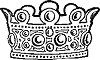
\includegraphics[width=2.7cm]{viking-tales/014}
\end{figure}

\chapter[\itshape A Reading List]{
    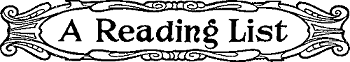
\includegraphics[width=9.3cm]{viking-tales/048}}

\subsection*{Geography}

NORWAY: ``The Earth and Its Inhabitants,'' Reclus. \emph{D. Appleton \&
Co., New York.}

\noindent ICELAND: ``The Earth and Its Inhabitants,'' ``Iceland,''
Baring-Gould. \emph{Smith, Elder \& Co., London, 1863.}

\begin{itemize}[itemsep=0pt]
\item ``Iceland, Greenland, and the Faroes.'' \emph{Harper Bros., New York.}
\item ``An American in Iceland,'' Kneeland. \emph{Lockwood, Brooke \& Co., Boston,
1876.}
\end{itemize}

\noindent GREENLAND: ``The Earth and Its Inhabitants,'' Reclus. \emph{D.
Appleton \& Co., New York.}

\begin{itemize}
\item ``Iceland, Greenland, and the Faroes.'' \emph{Harper Bros., New York.}
\end{itemize}

\subsection*{Customs}

``Viking Age,'' Du Chaillu. \emph{Charles Scribner's Sons, 1889.}

\noindent``Private Life of the Old Northmen,'' Keyser; translated by
Barnard. \emph{Chapman \& Hall, London, 1868.}

\noindent ``Saga Time,'' Vicary. \emph{Kegan Paul, Trench, Trübner \&
Co., London.}

\noindent ``Story of Burnt Njal'' (Introduction), Dasent. \emph{Edmonston
\& Douglas, Edinburgh, 1861.}

\noindent ``Vikings of the Baltic, a romance;'' Dasent. \emph{Edmonston
\& Douglas, Edinburgh.}

\noindent ``Ivar the Viking, a romance;'' Du Chaillu. \emph{Charles
Scribner's Sons, New York.}

\noindent ``Viking Path, a romance;'' Haldane Burgess. \emph{Wm.
Blackwood \& Sons, Edinburgh, 1894.}

\noindent ``Northern Antiquities,'' Percy, edited by Blackwell.
\emph{Bohn, London, 1859.}

\noindent Also the Sagas named on page 206.

\subsection*{Mythology}

The Prose Edda, ``Northern Antiquities,'' Percy, edited by Blackwell.
\emph{Bohn, London, 1859.}

\noindent ``Norse Mythology,'' Anderson. \emph{Scott, Foresman \& Co.,
Chicago, 1876.}

\noindent ``Norse Stories,'' Mabie. \emph{Rand, McNally \& Co., Chicago,
1902.}

\noindent ``Northern Mythology,'' Thorpe. \emph{Lumley, London, 1851.}

\noindent ``Classic Myths,'' Judd. \emph{Rand, McNally \& Co., Chicago,
1902.}

\subsection*{Incidents}

HARALD: Saga of Harald Hairfair, in ``Saga Library,'' Magnusson and
Morris, Vol. I. \emph{Bernard Quaritch, London; Charles Scribner's Sons,
New York, 1892.}

\noindent INGOLF: ``Norsemen in Iceland,'' Dasent in Oxford Essays, Vol.
IV. \emph{Parker \& Son, London, 1858.}

\begin{itemize}[itemsep=0pt]
\item ``Iceland, Greenland, and the Faroes.'' \emph{Harper Bros., New York.}
\item ``A Winter in Iceland and Lapland,'' \emph{Dillon. Henry Colburn, London,
1840.}
\end{itemize}

\noindent ERIC, LEIF, AND THORFINN: ``The Finding of Wineland the Good,''
Reeves. \emph{Henry Froude, 1890.}

\begin{itemize}
\item ``America Not Discovered by Columbus.'' Anderson. \emph{Scott, Foresman \&
Co., Chicago, 1891.}
\end{itemize}

\subsection*{Credibility of Story}

Winsor's ``Narrative and Critical History of America,'' Vol. I. \emph{C.
A. Nichols Co., Springfield, Mass., 1895.}

\noindent ``Discovery of America,'' Fiske, Vol. I. \emph{Houghton,
Mifflin \& Co., Boston, 1892.}

\subsection*{Other Sagas Easily Accessible}

``Saga Library,'' 5 vols.; Morris and Magnusson. \emph{Bernard Quaritch,
London; Charles Scribner's Sons, New York, 1892.} As follows:

\begin{itemize}[itemsep=0pt]
\item ``The Story of Howard the Halt,'' ``The Story of the Banded Men,'' ``The
Story of Hen Thorir.'' Done into English out of Icelandic by William
Morris and Eirikr Magnusson.
\item ``The Story of the Ere-dwellers,'' with ``The Story of the
Heath-slayings'' as Appendix. Done into English out of the Icelandic
by William Morris and Eirikr Magnusson.
\item ``The Stories of the Kings of Norway, called the Round World''
(Heimskringla). By Snorri Sturluson. Done into English by William
Morris and Eirikr Magnusson. With a large map of Norway. In three
volumes.
\end{itemize}

\noindent ``Gisli the Outlaw,'' Dasent. \emph{Edmonston \& Douglas,
Edinburgh.}

\noindent ``Orkneyinga Saga,'' Anderson. \emph{Edmonston \& Douglas,
Edinburgh.}

\noindent ``Volsunga Saga,'' Morris and Magnusson. \emph{Walter Scott,
London.}

\noindent ``The Younger Edda,'' Anderson. \emph{Scott, Foresman \& Co.,
Chicago, 1880.}

\noindent (A full bibliography of the Sagas may be found in ``Volsunga
Saga.'')

\begin{figure}[hb]
    \centering
    \vskip8pt
    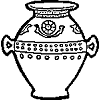
\includegraphics[width=2.7cm]{viking-tales/011}
\end{figure}

\chapter[\itshape A Pronouncing Index]{
    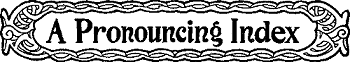
\includegraphics[width=9.3cm]{viking-tales/049}}

(\emph{This index and guide to pronunciation which are given to indicate
the pronunciation of the more difficult words, are based upon the 1918
edition of Webster's New International Dictionary.})

\noindent\textbf{Transcriber's Note:}\\
Minor typographical errors have been corrected without note. The up tack
diacritical mark over a vowel is represented by [+a], [+e], [+i] and
[+o].

\begin{multicols}{3}
\noindent\textbf{Aegir} (ē´ jĭr)\\
\textbf{\emph{Ȧ}rā´ bĭ \emph{ȧ}}\\
\textbf{Ärn´ vĭd}\\
\textbf{Ăs´ gärd}\\
\textbf{A̤ud´ bĭ ôrn}\\
\textbf{A̤u´dŭn}

\noindent\textbf{Bĭ är´ nĭ}

\noindent\textbf{Eric} (ē´ rĭk)\\
\textbf{Ericsson} (ĕr´ ĭk s\emph{ŭ}n)
\textbf{Eyjolf} (ī´ y{[}+o{]}lf)

\noindent\textbf{Faroes} (fā´ rōz)\\
\textbf{fiord} (fyôrd)\\
\textbf{Flō´ kĭ}

\noindent\textbf{Grĭm}\\
\textbf{Gŭd´ bränd}\\
\textbf{Gŭd´ rĭd}\\
\textbf{Gŭd´ rōd}\\
\textbf{Gŭn\emph{n}´ bĭ ôrn}\\
\textbf{Gṳ´ t\emph{h}ôrm}\\
\textbf{Gyda} (gē´ d{[}+a{]})

\noindent\textbf{Hä´ kĭ}\\
\textbf{Hä´ k{[}+o{]}n}\\
\textbf{Hälf´ dăn}\\
\textbf{Hăr´ ăld}\\
\textbf{Hä´ värd}\\
\textbf{Hĕl´ ä}\\
\textbf{Hĕl´ g{[}+a{]}}\\
\textbf{Hẽr´ st\emph{e}īn}\\
\textbf{Holmstein} (hōlm´ stīn)

\noindent\textbf{Ĭn´ gôlf}\\
\textbf{Ī´ vär}

\noindent\textbf{Leif} (l{[}+i{]}f)

\noindent\textbf{Niflheim} (n{[}+e{]}v´ 'l hām)

\noindent\textbf{Ō´ dĭn}\\
\textbf{Ō´ läf}\\
\textbf{Orkneys} (ôrk´ nĭz)

\noindent\textbf{Rän}\\
\textbf{Reykjavik} (rā´ ky\emph{ȧ} vēk´)\\
\textbf{Rôlf}

\noindent\textbf{Shĕt´ l\emph{ă}nds}\\
\textbf{Sif} (sēf)\\
\textbf{Sighvat} (sĭg´ văt)\\
\textbf{Snorri} (snŏr´ r{[}+e{]})\\
\textbf{Sôl´ fĭ}

\noindent\textbf{Thor (thôr)}\\
\textbf{T\emph{h}ôr´ bĭ ôrn}\\
\textbf{T\emph{h}ôr´ fĭnn}\\
\textbf{T\emph{h}ôr´ gĕst}\\
\textbf{T\emph{h}ôr´hĭld}\\
\textbf{T\emph{h}ôr´ kĕl}\\
\textbf{T\emph{h}ôr´ l\emph{e}īf}\\
\textbf{T\emph{h}ôr´ ôlf}\\
\textbf{T\emph{h}ôr´ st\emph{e}īn}\\
\textbf{Tyrker} (tẽr´ kẽr)

\noindent\textbf{Văl hăl´ \emph{lȧ}}\\
\textbf{Valkyria} (văl kĭr´ \emph{yȧ})\\
\textbf{Vī´ kĭng}
\end{multicols}

\subsection*{A Guide to Pronunciation}

\begin{multicols}{3}
\noindent\textbf{ā} as in \textbf{āle}\\
\textbf{ă} as in \textbf{ădd}\\
\textbf{\emph{ă}} as in \textbf{fin\emph{ă}l}\\
\textbf{ȧ} as in \textbf{ȧsk}\\
\textbf{\emph{ȧ}} as in \textbf{sof\emph{ȧ}}\\
\textbf{ä} as in \textbf{ärm}\\
\textbf{a̤} as in \textbf{a̤ll}

\noindent\textbf{ē} as in \textbf{ēve}\\
\textbf{{[}+e{]}} as in \textbf{{[}+e{]}vent´}\\
\textbf{ĕ} as in \textbf{ĕnd}\\
\textbf{ẽ} as in \textbf{hẽr}

\noindent\textbf{ī} as in \textbf{īce}\\
\textbf{ĭ} as in \textbf{ĭt}

\noindent\textbf{ō} as in \textbf{ōld}\\
\textbf{{[}+o{]}} as in \textbf{{[}+o{]}bey´}\\
\textbf{ŏ} as in \textbf{ŏdd}\\
\textbf{ô} as in \textbf{lôrd}

\noindent\textbf{ŭ} as in \textbf{ŭp}\\
\textbf{\emph{ŭ}} as in \textbf{circ\emph{ŭ}s}\\
\textbf{ṳ} as in \textbf{rṳde}

\noindent\textbf{ȳ} as in \textbf{flȳ}
\end{multicols}

\noindent Silent letters are italicized.
